\documentclass{article}
\usepackage{graphicx} % Required for inserting images
\usepackage[ruled,vlined]{algorithm2e, setspace}
\usepackage{amsthm, amssymb, amsmath}

\begin{document}

\section{Extra files}

\begin{figure}[htbp]
    \centering
    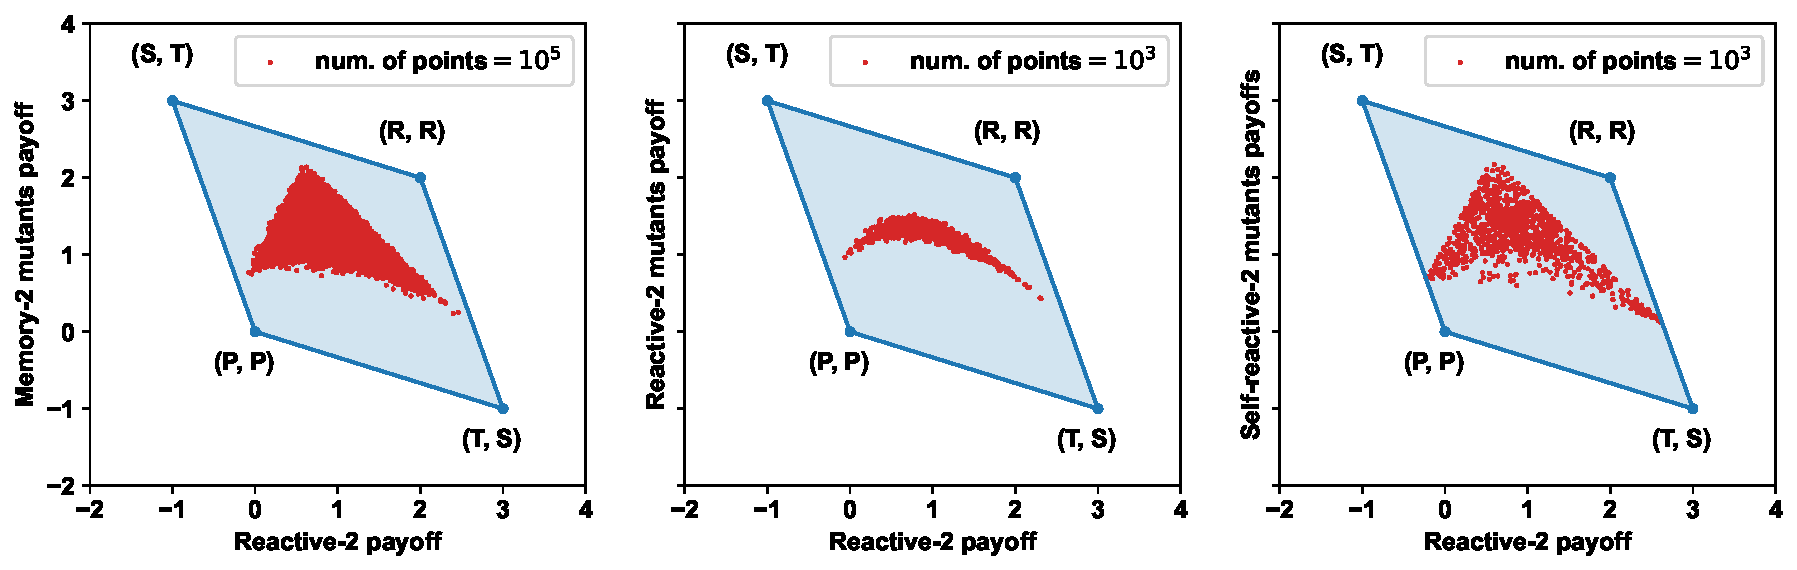
\includegraphics[width=\textwidth]{figures/sufficiency_of_self_reactive_numerical_example_n_2.pdf}
    \caption{Parameters: $b=3, c=1$ and $\mathbf{p}=(0.37, 0.89, 0.95, 0.23)$}
    \label{fig:enter-label}
\end{figure}


\begin{algorithm}[H]
\setstretch{1.35}
  \SetKwInOut{Input}{input}
  \Input{$\mathbf{p}, n$}
   $L(\mathbf{p}) \gets \left\{\mathbf{\tilde{p}} \in \{0, 1\}^{2 ^ n} ~\big|~ 
   s_{\mathbf{\tilde{p},\mathbf{p}}} \geq s_{\mathbf{p}, \mathbf{p}} \right\}$\;
  \uIf{$ L(\mathbf{p}) = \emptyset $}{
    isNash $\leftarrow$ True \;
  }
  \Else{
    isNash $\leftarrow$ False \;
  }
  \Return (\(\mathbf{p}\), isNash) \;
  \caption{Nash Evaluation for reactive$-n$ strategies.}
\end{algorithm}

\end{document}
